\documentclass[a4paper,12pt]{article}
%%%%%%%%%%%%%%%%%%%%%%%%%%%%%%%%%%%%%%%%%%%%%%%%%%%%%%%%%%%%%%%%%%%%%%%%%%%%%%%%%%%%%%%%%%%%%%%%%%%%%%%%%%%%%%%%%%%%%%%%%%%%%%%%%%%%%%%%%%%%%%%%%%%%%%%%%%%%%%%%%%%%%%%%%%%%%%%%%%%%%%%%%%%%%%%%%%%%%%%%%%%%%%%%%%%%%%%%%%%%%%%%%%%%%%%%%%%%%%%%%%%%%%%%%%%%
\usepackage{eurosym}
\usepackage{vmargin}
\usepackage{amsmath}
\usepackage{graphics}
\usepackage{epsfig}
\usepackage{enumerate}
\usepackage{multicol}
\usepackage{subfigure}
\usepackage{fancyhdr}
\usepackage{listings}
\usepackage{framed}
\usepackage{graphicx}
\usepackage{amsmath}
\usepackage{chngpage}
%\usepackage{bigints}

\usepackage{vmargin}
% left top textwidth textheight headheight
% headsep footheight footskip
\setmargins{2.0cm}{2.5cm}{16 cm}{22cm}{0.5cm}{0cm}{1cm}{1cm}
\renewcommand{\baselinestretch}{1.3}

\setcounter{MaxMatrixCols}{10}

\begin{document}
\Large 

\noindent In a very small empirical study a sample from a random variable $X$ is observed. 
The data can be entered into R using the following code:


\begin{framed}\begin{verbatim}
x <- c(0.22, 0.38, 1.28, 0.54, 0.56, 1.36,
       0.55, 0.37, 0.43, 0.46, 0.62, 0.54,
       0.54, 0.51, 0.44, 0.68, 0.55, 0.30)
\end{verbatim} \end{framed}

\medskip 
\subsection*{Exercise 1} 
\noindent Estimate the expected value of $X$.


\begin{framed}\begin{verbatim}
mean(x)
\end{verbatim} \end{framed}

\begin{verbatim}
0.573888
\end{verbatim}


%%%%%%%%%%%%%%%%%%%%%%%%%%%%%%%%%%%%%%%%%%%%%55
\newpage
\subsection*{Exercise 2} 
\noindent Calculate a 95\% confidence interval for the expected value of $X$, assuming that $X$ is Normally distributed.

\begin{framed}\begin{verbatim}
t.test(x, conf=0.95)
\end{verbatim} \end{framed}
\begin{verbatim}
    	One Sample t-test
    
    data:  x
    
    t = 8.2805, df = 17, p-value = 2.276e-07
    alternative hypothesis: true mean is not equal to 0
    
    95 percent confidence interval:
     0.4276654 0.7201123
    
    sample estimates:
    mean of x 
    0.5738889 
    
\end{verbatim}
\newpage 

\noindent \textbf{Shapiro-Wilk normality test}

\begin{framed}\begin{verbatim}
> shapiro.test(x)

	Shapiro-Wilk normality test

data:  x
W = 0.745, p-value = 0.00028
\end{verbatim} \end{framed}

\newpage 
\begin{framed}\begin{verbatim}

qqnorm(x, cex=1.5, pch=18, col="black" )

qqline(x ,lwd=2,col="red")

\end{verbatim} \end{framed}

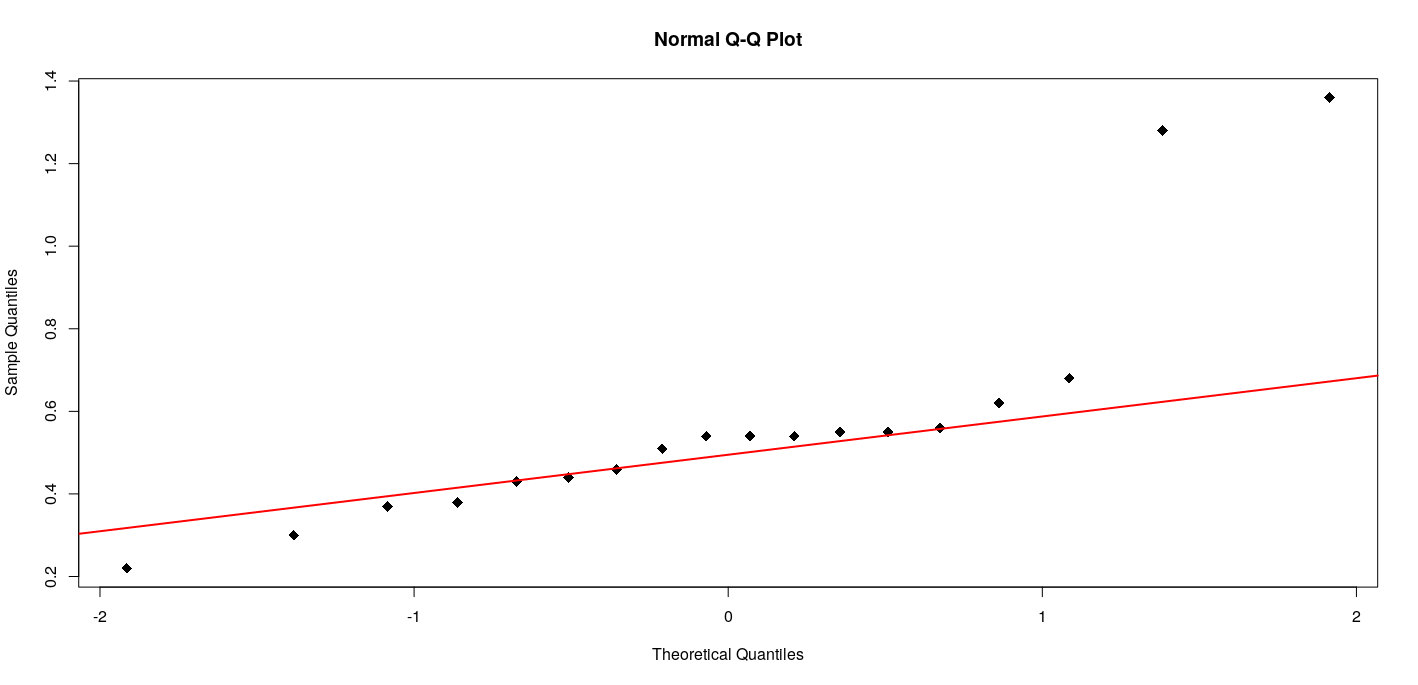
\includegraphics[scale=0.45]{00-C1/images/00-C1-Q1-qqnorm.png}
\newpage 

\noindent \textbf{Tidyverse}

\begin{framed}\begin{verbatim}

# install.packages(c("magrittr","broom"))

library(magrittr)
library(broom)

t.test(x, conf=0.95) %>% tidy()


\end{verbatim} \end{framed}




%%%%%%%%%%%%%%%%%%%%%%%%%%%%%%%%%%%%%%%%%%%%%55
\newpage

\subsection*{Exercise 3}

\noindent Construct a confidence interval for the expected value of $X$ using the bootstrap
method with 10,000 bootstrap replications.

\begin{framed}
\begin{verbatim}
> 1:4
[1] 1 2 3 4
> 1:5
[1] 1 2 3 4 5
> 1:6
[1] 1 2 3 4 5 6
>
> sample(1:4,replace =TRUE)
[1] 1 1 4 1
>
> sample(1:5,replace =TRUE)
[1] 5 3 1 5 4
>
> sample(1:6,replace =TRUE)
[1] 4 2 1 2 2 4

\end{verbatim}
\end{framed}
\begin{framed}\begin{verbatim}
replicate(10, mean(sample(x,replace =TRUE)))
\end{verbatim} \end{framed}


\begin{verbatim}
 [1] 0.5927778 0.4955556 0.5144444 0.5444444 0.6272222
 [6] 0.5577778 0.5438889 0.4916667 0.6233333 0.6266667    
\end{verbatim}




\begin{framed}\begin{verbatim}
y = replicate(10000,mean(sample(x,replace =TRUE))) 

quantile(y,prob=c(0.025,0.975)) 

\end{verbatim} \end{framed}


\begin{verbatim}
     2.5%     97.5% 
0.4544444 0.7222222 
\end{verbatim}

%%%%%%%%%%%%%%%%%%%%%%%%%%%%%%%%%%%%%%%%%%%%%55
\newpage


\subsection*{Exercise  4}

\noindent Comment on the differences between the confidence intervals in exercises 2 and 3.


\begin{itemize}
    \item The CIs are almost identical with the CI in exercise 3 being narrower. 
    \item The reason might be that the distribution of $X$ is not normal, and therefore the
distribution of the mean is not normal for the small sample size we have in this
question. 
    \item 


The bootstrap method provides a good approximation of the distribution of the mean
independently of the type of distribution.
\end{itemize}



\end{document}

